\chapter{Feature extraction} % (fold)
\label{chap:feature_extraction}
This chapters describes different approaches on the marker detection. It explains the trade-offs,methods that have been considered and applied for the different markers. The markers that have been analysed and detected in this project are Marker 1 (Color), Marker 2 (Thin lines) and Marker 3 (Corny). 

It is a trade-off between speed (how many detections per second) and precision (how precise the detection is). It is necessary to know whether a fast or a slowly moving object is being tracked. There are several options available. As more features are added to the code, runtime is likely to become longer. The runtime also depends on the computational capability of the computer.

Another trade-off lies in the universality of the detection - whether the detection is effective in a closed artificial environment (easier to detect) or in real "chaotic" environment (the simple methods may fail).

\newpage
%\begin{figure}[!ht]
%	\centering
%	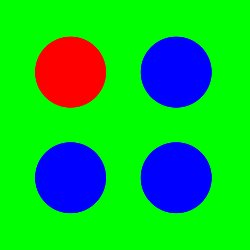
\includegraphics[width=0.01\textwidth]{figures/Marker1.jpg}
%	\caption{Marker 1 Color}
%	\label{fig:markerColor}
%\end{figure}
\section{Marker 1 (Color)} 
Here goes first marker

\newpage
\section{Marker 2 (2a Thin lines)}

\newpage
\section{Marker 3 (Corny)}
% chapter featre_extraction (end)